\chapter{Método de trabajo}
\label{chap:metodo}

\noindent
\drop{A}{} lo largo de este capítulo se planteará la metodología escogida para el desarrollo de este proyecto, justificando su elección y explicando sus principales características así como el  primer planteamiento para afrontar el problema. También se mencionarán las herramientas software y hardware empleadas en la realización tanto del proyecto como de esta documentación.


\section{Metodología de desarrollo}

Para la realización de este proyecto se ha escogido una metodología ágil \cite{ilieva2004analyses}, en concreto se va a aplicar el marco Scrum \cite{schwaber2004agile}. Las metodologías ágiles se caracterizan por el desarrollo del proyecto mediante interacciones incrementales que finalizan con un entregable, el cual aporta una determinada funcionalidad de manera que pueda ser evaluado por el usuario. Mediante estos entregables tempranos se pretende reducir el riesgo de desarrollar un producto que no se ajuste a las necesidades del usuario, permitiendo añadir cambios y adaptarse a los requisitos de este durante su desarrollo.

\subsection{Scrum}

Scrum es un marco de desarrollo ágil basado en ciclos de desarrollo iterativos e incrementales para la gestión y desarrollo de proyectos. Scrum establece un conjunto de prácticas y roles que se deberán emplear en el desarrollo de un proyecto con el objetivo de minimizar los riesgos que conlleva este desarrollo. Una de las principales características de este modelo, es que se busca el desarrollo colaborativo, en el que todo el equipo trabaja de manera autoorganizada y sin la intervención de agentes externos al proyecto o producto que se desea desarrollar. El equipo de desarrollo de Scrum debe trabajar de manera muy cercana, comunicándose entre sí continuamente, y realizando revisiones de todo lo que se ha desarrollado con gran frecuencia para asegurar la mayor calidad posible del producto. Debido a su capacidad de adaptabilidad a las necesidades del usuario y a los cambios, es especialmente útil en entornos donde existe volatilidad en las necesidades de los usuarios, y donde se necesitan obtener resultados tangibles en un tiempo corto. 

Como se ha mencionado anteriormente \textit{``Scrum no es un proceso o una técnica para la creación de productos; si no un marco dentro del cual puedes emplear diferentes técnicas y procesos''} \footnote{http://www.scrumguides.org/scrum-guide.html}. Scrum está fundamentalmente basado en el enfoque empírico, revisando continuamente el trabajo que se ha llevado a cabo para mejorar. Está basado principalmente en tres pilares. Por un lado encontramos la \textbf{transparencia}, que implica que todos los aspectos importantes del proyecto deben ser conocidos por todos los integrantes del equipo Scrum, y que además deben existir estándares conocidos y seguidos por los implicados, de manera que todos los integrantes entiendan aquello que se está representando. Por otro lado debe existir una \textbf{inspección}, que pese a que no debe ser tan frecuente que se interponga en el desarrollo del trabajo, debe ser suficiente como para asegurar que el producto se desarrolla con la calidad adecuada. Finalmente, el marco Scrum y especialmente el equipo que implementa dicho marco, deben ser capaces de \textbf{adaptarse} a los cambios que tras las inspecciones se consideren necesarios para asegurar el correcto desarrollo del producto.

\subsubsection{Roles en Scrum}

Como se ha mencionado anteriormente, solo aquellos miembros que se encuentren dentro del proyecto serán los encargados de tomar decisiones que afecten a dicho proyecto, sin intervención de terceras personas ajenas a este. Así pues, el equipo de Scrum es auto-suficiente y auto-organizado, y es este equipo el encargado de tomar todas las decisiones que afecten a este desarrollo. Scrum define tres grandes roles dentro de su estructura, tal y como se muestra en la Figura \ref{fig:scrum-roles}, aunque luego pueda existir una distribución más amplia dentro de estos.

\begin{itemize}
\item \textbf{Product Owner (Propietario del producto):} Es la persona que representa al cliente y a los stakeholders (o personas interesadas en el producto). Es el encargado de maximizar el valor del producto, asegurándose de que las necesidades se cumplen de la manera más exitosa posible. Para se encarga de redactar las Historias de usuario, dotarlas de prioridad y añadirlas al Product Backlog.

\item \textbf{Scrum Master (Facilitador):} Es el encargado de facilitar la realización del proyecto por parte del equipo. Debido a la característica autoorganizativa de Scrum no representa el papel clásico de líder de proyecto, sino que actúa como facilitador del equipo, eliminando o minimizando aquellos obstáculos que puedan perjudicar al desarrollo del proyecto. También es el encargado de hacer cumplir el marco de Scrum, así como de liderar o dirigir las reuniones para asegurarse de que son productivas y se desarrollan mediante la idelogía Scrum. Ayuda al Product Owner en la realización del Product Backlog, de manera que se tenga claro que elemento es necesario desarrollar a continuación para que el equipo pueda seguir trabajando continuamente.

\item \textbf{Development Team (Equipo de desarrollo):} Este equipo es el encargado de materializar las historias de usuario y las necesidades del proyecto en entregables iterativos ya finalizados para que sean evaluados. Dentro de este equipo debe haber personas con las capacidades adecuadas para el desarrollo de todas las funcionalidades necesarias en cada incremento. Debido a esto los equipos se componen de personal con capacidades variadas y complementarias. Estos equipos deben ser de un tamaño reducido de manera que la autoorganización pueda funcionar, y pueda existir una gran comunicación entre el equipo. 
\end{itemize} 

\begin{figure}[!h]
\begin{center}
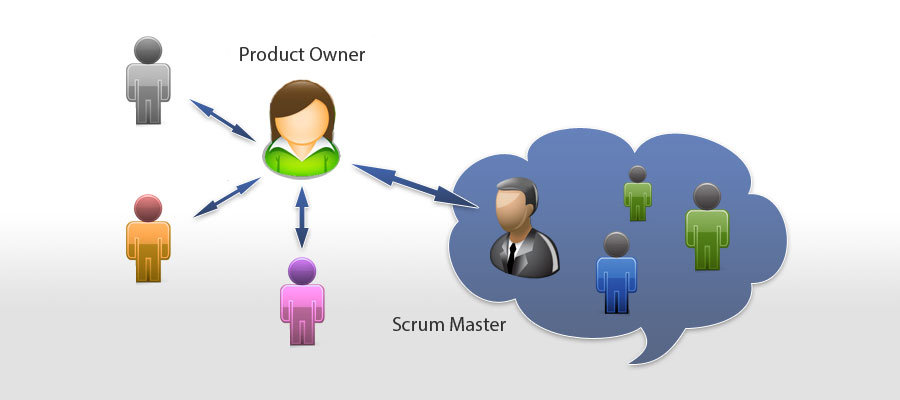
\includegraphics[width=0.8\textwidth]{./figures/scrum-roles.jpg}
\caption[Roles en Scrum]{Roles en Scrum. Fuente: \href{https://www.scrum.as/}{https://www.scrum.as/}}
\label{fig:scrum-roles}
\end{center}
\end{figure}

\subsubsection{Sprint}

El Sprint es la piedra angular en Scrum. Representa un bloque de tiempo de una a cuatro semanas, que debe finalizar con la entrega de un elemento incremental que aporte funcionalidad y que pueda ser evaluado.

\subsubsection{Eventos}

Del concepto de Sprint se derivan una serie de eventos relacionados con este. En la 
Figura \ref{fig:scrum-framework} se puede observar el esquema que se seguiría para cada Sprint.
\begin{itemize}
\item \textbf{Sprint Planning Meeting (Reunión de planificación del Sprint):} Esta reunión se lleva a cabo al comienzo de cada Sprint, y en ella se decide como se va a organizar el Sprint, estableciendo que elementos del Product Backlog se van a desarrollar, así como periodos y plazos. La duración máxima es de unas cuatro horas para los Sprint de 2 semanas y ocho para los Sprint de un mes.
\item \textbf{Daily Scrum (Scrum Diario):} Durante esta reunión diaria de unos quince minutos aproximadamente, se evalúa el trabajo realizado desde el ultimo Daily Scrum, se plantea el objetivo para ese día, y se evalúan los posibles problemas o dificultades que puedan afectar a la consecución del objetivo.
\item \textbf{Sprint Review (Revisión del Sprint):} Este evento se realiza cada vez que se finaliza un Sprint, y durante esta revisión se evalúa el trabajo realizado y se presentan los avances al cliente o stakeholders.
\item \textbf{Sprint Retrospective (Retrospectiva de Sprint):} Durante este evento el equipo evalúa aquello que se hizo mal o puede mejorarse, y se ponen en marcha las medidas necesarias para solventar los errores o implementar las mejoras necesarias. Es una revisión que se realiza tras el Sprint Review y antes de que se comience con el siguiente Sprint.
\end{itemize}

\begin{figure}[!h]
\begin{center}
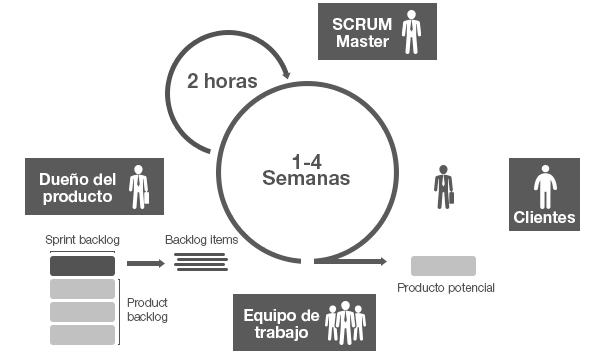
\includegraphics[width=1\textwidth]{./figures/scrum-framework.jpg}
\caption[Esquema de la estructura un Sprint]{Esquema de la estructura un Sprint. Fuente: \href{http://www.i2btech.com/}{http://www.i2btech.com/}}
\label{fig:scrum-framework}
\end{center}
\end{figure}

\subsubsection{Artefactos}

Los artefactos en Scrum ayudan al equipo a la consecución de los objetivos y a la planificación y estructuración de estos, permitiendo proporcionar la transparencia necesaria para que todos puedan tener una imagen de lo que se necesita, y de la situación del proyecto, permitiendo una adaptación y mejora continua.

\begin{itemize}
\item \textbf{Product Backlog (Lista de Producto):} El Product Backlog contiene todos los elementos necesarios bien sean características como fallos por resolver, requisitos no funcionales, mejoras o cualquier otro elemento que sea necesario llevar a cabo para lograr llevar a cabo el proyecto. Es visible a todo el equipo, pero solo podrá ser cambiado con el consentimiento del Product Owner. Los items que conforman esta lista se ordenan en función de la prioridad para su resolución, y deben contener además, una estimación del tiempo necesario para llevar dicha tarea o elemento a cabo. Es necesario explicar en que consisten los items que se añaden a esta lista, que pese a que no es obligatorio que sean de un formato concreto, suelen consistir en Historias de Usuario o \acs{HU}. Estas \acs{HU} describen una necesidad, funcionalidad o característica, que el sistema deberá contener para su desarrollo exitoso. Contienen únicamente aquello que debe hacerse, pero no el cómo, y deben ser lo suficientemente claras y cortas como para ser fácilmente entendibles. Un ejemplo de plantilla para estas \acs{HU} se definió como \textit{Como <role>, quiero <objetivo/deseo> para <beneficio>}. También se ha remarcado la posibilidad de suprimir la parte del \textit{para} cuando no sea necesario o no aporte nada de utilidad. 

\item \textbf{Sprint Backlog (Lista de tareas pendientes del Sprint):} Esta lista contiene aquellas tareas que se han seleccionado del Product Backlog para su desarrollo en el Sprint actual. Estas historias se pueden desglosar en tareas a las que se les asigna un tiempo de realización. Generalmente se suele utilizar un mecanismo que se puede implementar mediante una pizarra o mediante herramientas más complejas como herramientas software, en el que se clasifican las tareas o historias según su situación actual dentro del Sprint como \textit{to do} si aún no se ha empezado a trabajar en ella, \textit{in progress} si se está trabajando y \textit{done} si está completa.
\end{itemize}

\subsection{Aplicación al proyecto} 

Siendo el marco explicado anteriormente el elegido para el desarrollo de este proyecto, es el momento de explicar como se ha planteado este proyecto de acuerdo al marco Scrum.
En primer lugar es preciso identificar al equipo Scrum, el cual pese a no ser recomendable el hecho de que el Scrum Master y el Product Owner sean la misma persona, debido al carácter docente de este trabajo era la única solución. Así pues, el equipo queda de la siguiente manera:
\begin{itemize}
\item Product Owner: Jesús Serrano Guerrero
\item Development Team: Victor Gualdras de la Cruz
\item Scrum Master: Jesús Serrano Guerrero
\end{itemize}

En segundo lugar, se precisa la realización de una primera versión del Product Backlog tal y como se muestra en la Figura \ref{tab:user-stories} de manera que el grupo de desarrollo pueda comenzar a trabajar en el proyecto. En esta tabla, las historias de usuario se encuentran ordenadas según la prioridad que tienen para el proyecto. Esto quiere decir que se tendrán que desarrollar en el orden establecido, debido a que son las que mayor valor aportan al negocio, y son necesarias para las siguientes tareas.

\begin{table}[hp]
  \centering
  {\small
  \begin{tabular}{p{.10\textwidth}p{.15\textwidth}p{.30\textwidth}p{.10\textwidth}p{.10\textwidth}}
  \tabheadformat
  \tabhead{Identificador}   &
  \tabhead{Como}      &
  \tabhead{Quiero/Necesito} &
  \tabhead{Estimación} &
  \tabhead{Situación} \\
\hline
HU & Usuario & Acceder a una aplicación de mensajería &  & To Do \\
\hline
HU & Usuario & Poder realizar la entrada en el chat mediante texto y mediante voz & & To Do \\
\hline
HU & Usuario & Conocer cual de mis contactos utiliza la aplicación & & To Do \\
\hline
HU & Usuario & Comunicarme con otros usuarios & & To Do \\
\hline
HU & Usuario & Poder enviar imágenes a otros usuarios & & To Do \\
\hline
HU & Usuario & Realizar búsquedas de imágenes filtrando mediante mi entrada & & To Do \\
\hline
HU & Usuario & Que se me muestren aquellas imágenes que mas se adapten a mis gustos & & To Do \\
\hline
HU & Usuario & Que la búsqueda no quede limitada a mi entrada, sino a su semántica & & To Do \\
\end{tabular}

  }
  \caption[Primera versión del Product Backlog]
  {Primera versión del Product Backlog}
  \label{tab:user-stories}
\end{table}






\section{Herramientas utilizadas}

En esta sección se trataran las principales herramientas utilizadas para el desarrollo de este proyecto, tanto hardware como software, incluyendo las \acs{API}s más importantes.

\subsection{Herramientas Hardware}

A continuación se muestran los dispositivos hardware utilizados en el desarrollo de este \ac{TFG}
\begin{itemize}
\item Ordenador portátil personal sobre el que se realizará el desarrollo del proyecto.
\item Dos dispositivos Smartphone con Sistema Operativo Android sobre los que se realizarán las pruebas.
\end{itemize}

\subsection{Herramientas Software}

Las herramientas software más importantes empleadas en este proyecto se muestran a continuación.

\subsubsection{Lenguajes de programación}

\textbf{Java}

El lenguaje de programación Java\footnote{https://www.oracle.com/es/java/index.html} es un lenguaje de propósito general y alto nivel, cuyas principales características son las de ser \ac{OO}. Además, el código generado por Java tiene la característica de que una vez compilado puede ejecutarse en cualquier plataforma que que soporte Java.

Java será el principal lenguaje en el que se desarrolle la aplicación Android, ya que es el lenguaje sobre el que funcionan las aplicaciones para esta plataforma. Si bien se usará algún otro lenguaje como XML para las interfaces, Java es el más importante.

\textbf{Python}

Python\footnote{https://www.python.org/} es un lenguaje interpretado de alto nivel, que al igual que java es de propósito general. Ofrece la generación de código generalmente más breve que otro que cumpla el mismo propósito en otros lenguajes, y es comúnmente utilizado como lenguaje de prototipado rápido. 

Será utilizado para el desarrollo del servidor de este proyecto debido a su facilidad y potencia de uso en el ámbito de las comunicaciones, y especialmente por su fácil integración con \acf{GCP}.

\textbf{LaTeX}

LaTeX \footnote{https://www.latex-project.org/} es un procesador de textos para la preparación de documentos de gran calidad de tipografía especialmente diseñado para redactar documentos que pretenden ser publicados en algún medio, especialmente largos artículos técnicos o científicos. Permite que el escritor pueda centrarse en lo que escribe y no en el formato y el diseño que debe tener el texto, encargándose LaTeX de esto. Este será el lenguaje utilizado para la redacción de este documento.

\textbf{JSON}

JSON que son las siglas para JavaScript Object Notation, es un lenguaje de formato para el intercambio de datos\footnote{http://www.json.org/}. Está basado en un conjunto del lenguaje de programación JavaScript, y se compone principalmente de dos estructuras de alto nivel, una tupla de nombre valor, y una lista de atributos. Dentro de los atributos que se pueden encontrar en el valor de las tuplas encontramos los datos primitivos característicos de todo lenguaje de programación como cadenas, números, y valores booleanos, así como el elemento nulo. Este será el formato que se usará principalmente para la transmisión y comunicación de datos a través de la red.


\subsubsection{Android Studio}

Como se mencionó en la sección \ref{chap:intro}, se pretende desarrollar una aplicación para dispositivos Smartphones con \acs{SO} Android, y por tanto es recomendable disponer de un \acs{IDE} que nos ayude en esta tarea, y uno de estos entornos es Android Studio\footnote{https://developer.android.com/studio/index.html}. Pese a que existen otros entornos de desarrollo que nos pueden ayudar también para este propósito, como Eclipse utilizando el plugin Android Developments Tools \footnote{https://marketplace.eclipse.org/content/android-development-tools-eclipse}, se ha decidido utilizar Android Studio debido a ser el \acs{IDE} oficial para el desarrollo de aplicaciones Android y por tanto, proporcionar la seguridad de que siempre estará actualizado y contendrá todo lo necesario para poder desarrollar estas aplicaciones, y además por la gran lista de funcionalidades y facilidades que aporta. Algunas de estas utilidades son su integración con Gradle\footnote{https://gradle.org/} para la gestión de dependencias, la automatización de la compilación y el despliegue de las aplicaciones, un editor de código inteligente y auto completado, emulador integrado, herramientas que ayudan al depurado y al testing, y muchas otras opciones como la integración con sistemas de control de versiones.

\begin{figure}[!h]
\begin{center}

\includegraphics[width=0.5\textwidth]{./figures/android-studio.png}
\caption{Android Studio logo}
\label{fig:android-studio}
\end{center}
\end{figure}

\subsubsection{Google Cloud Platform}
\label{GCP}

Google Cloud Platform o \acs{GCP} es una plataforma de computación en la nube \cite{CloudComputing} que ofrece diversos servicios de Infrastructure as a Service, Platform as a Service y Software as a Service. Estos servicios ofrecen características de escalabilidad, control automático y gestión de los recursos, herramientas de monitorización y sobre todo la simulación o virtualización de recursos hardware sin la necesidad de adquirirlos. Esta última característica es una de las principales para que este tipo de tecnología haya sido seleccionada. Esto permite que no sean necesarias tareas de mantenimiento del hardware, debido a que no habrá necesidad alguna de adquirir hardware específico para el servidor, que no haya que preocuparse por el consumo de energía, o de otras tareas de mantenimiento. Tampoco será necesario preocuparse por la infrautilización de recursos, o la necesidad repentina de tener que aumentar la potencia de procesamiento o almacenamiento según la demanda, ya que esta herramienta permite adaptarse con bastante facilidad a estos eventos. Estos servicios se conocen como \acs{IaaS}.

Además de estos servicios de virtualización de recursos, Google Cloud Platform también proporciona como se ha mencionado anteriormente servicios de \acs{PaaS}. Entre esos servicios se encuentran herramientas tanto para el desarrollo como el despliegue o el mantenimiento del software que se ejecutará en el servidor, además de la posibilidad de monitorizar tanto el tráfico como los datos que se encuentren almacenados en este. Es decir, pone gran cantidad de recursos al alcance del desarrollador y el equipo en general sin que este necesite tener que implementar e integrar por si mismo todos estos servicios. Ofrece también mecanismos para acceder a los servicios que se encuentren desplegados bajo los servidores.

Además de todo lo mencionado anteriormente, \acs{GCP} ofrece la posibilidad de utilizar herramientas software ya desarrolladas de manera que no sea necesario invertir tiempo en desarrollar utilidades que ya existen y que se pueden utilizar mediante el alquiler de ese servicio. Estos servicios son conocidos como \acs{SaaS}, y nos permite utilizar software de terceros para nuestras necesidades.


\begin{figure}[!h]
\begin{center}

\includegraphics[width=0.5\textwidth]{./figures/GCP.png}
\caption{Google Cloud Platform logo}
\label{fig:android-studio}
\end{center}
\end{figure}

De la gran cantidad de recursos que ofrece \acs{GCP} se explicarán los siguientes por ser los más relevantes en el desarrollo de este \ac{TFG}. A pesar de ello, se han usado otras herramientas y características que proporciona esta herramienta como los registros o el panel de control de \acs{API}s.

%TODO App Engine


\textbf{Google App Engine}

App Engine es el servicio \ac{PaaS} de Google, y permite almacenar y desplegar servicios web que serán gestionados en servidores propios de Google. Una de las grandes ventajas que proporciona es la de desarrollar aplicaciones que escalan automáticamente, además de numerosos servicios entre los que se encuentra los que se verán a continuación, como son el Datastore o el Blobstore.

\textbf{Google Cloud Datastore}

Google Cloud Datastore\footnote{https://cloud.google.com/datastore/docs/} es una base de datos NoSQL creada para escalar de manera automática, presentar un alto rendimiento y facilitar el desarrollo de aplicaciones. Los datos que se encuentran en el Datastore son accedidos mediante las denominadas \textit{transacciones}, que cumplen las características \acs{ACID} de atomicidad, consistencia, aislamiento y persistencia. Ofrece consistencia fuerte cuando se trata de operaciones que se realizan mediante claves y ancestros, y consistencia eventual en el resto de los casos. Estas transacciones también ofrecen toda las operaciones \acs{CRUD} de crear, leer, actualizar y eliminar. Google Datastore proporciona numerosos mecanismos para realizar estas transacciones, desde una librería JSON, clientes de código abierto o herramientas mantenidas por los usuarios como NDB o Objectify. Además de las características \acs{ACID}, ofrece también:

\begin{itemize}
\item Disponibilidad: Usa replicación para minimizar el impacto de que uno de los puntos en los que se encuentre falle.
\item Escalabilidad: Usa una arquitectura distribuida que maneja de manera automática el escalado.
\item Rendimiento: A la vez que es escalable es capaz de mantener un alto rendimiento gracias a su combinación de índices. En una consulta, su rendimiento depende del resultado de la consulta y no del tamaño total del conjunto de datos.
\item Almacenamiento y consultas flexibles: Es capaz de trasladar objetos y entidades propias de los lenguajes orientados a objetos y de script a entidades de manera muy natural. También provee de un lenguaje similar a SQL para realizar consultas.
\item Encriptación: Se encriptan los datos previo a su almacenado y se desencriptan antes de leídas por los usuarios.
\item Administración automática: Google se encarga de todo el mantenimiento.
\end{itemize} 

Como se ha mencionado anteriormente, Cloud Datastore es una base de datos NoSQL y que no se corresponde con el sistema relacional de gestión de base de datos. Existen algunas diferencias ya en los conceptos que estos tratan como se puede apreciar en el Cuadro \ref{tab:datastore-rdbms}. A diferencia de las filas de una misma tabla en los sistemas relacionales, una entidad de Google Datastore puede tener diferentes campos respecto a otra entidad del mismo tipo, o pueden tener propiedades con el mismo nombre y tipos diferentes. 

\begin{table}[hp]
  \centering
  {\small
  \begin{tabular}{p{.3\textwidth}p{.25\textwidth}p{.25\textwidth}}
  \tabheadformat
  \tabhead{Concepto}   &
  \tabhead{Google Datastore}      &
  \tabhead{\acs{RDBMS}} \\
\hline
Categoría del objeto & Kind/Tipo & Table/Tabla \\
\hline
Objeto único & Entity/Entidad & Row/Fila \\
\hline
Identificador único de objeto & Key/Clave & Primary Key/Clave Primaria \\
\hline
Dato individual sobre un objeto & Property/Propiedad & Field/Campo \\
\end{tabular}

  }
  \caption[Diferencia entre Google Datastore y los \acs{RDBMS}]
  {Diferencia entre Google Datastore y los \acs{RDBMS}}
  \label{tab:datastore-rdbms}
\end{table}

Otras diferencias notables con las bases de datos relacionales son su capacidad de escalado automática, capacidad de balanceo y distribución de datos para mejorar el rendimiento, las únicas consultas que permite son aquellas que permiten que su rendimiento solo dependa del tamaño del resultado proporcionado por la consulta, siendo independiente el número de entidades que existan en total. Esta última es una de las razones por las que algunas operaciones no existen en este sistema.

También es importante destacar que soporta multitud de tipos para sus propiedades, pudiendo incluso contener propiedades estructuradas compuestas por entidades de otros tipos.

Google Datastore se utilizará para almacenar los datos relativos a los usuarios que resulten de interés para la aplicación así como información referente a las imágenes para posteriormente poder ser utilizada en el sistema de recomendación.


\textbf{Google Cloud Blobstore}

Blobstore\footnote{https://cloud.google.com/appengine/docs/python/blobstore/} es un servicio proporcionado por Google Cloud Platform y que accedido mediante una \acs{API} disponible en los lenguajes Python, Java y Go permite almacenar ficheros de un tamaño superior al permitido por el servicio de Google Datastore. Los ficheros se suben en forma de blobs, los cuales se crean indirectamente. En primer lugar  es necesario solicitar mediante una llamada a la \acs{API} la generación de una \acs{URL}, posteriormente la aplicación cliente podrá proceder a la subida del archivo mediante un formulario web o algún otro tipo de petición \acs{HTTP} POST. Tras enviar el formulario con el fichero, el servicio Blobstore almacena el archivo y genera una clave para poder recuperar posteriormente el archivo almacenado en el blob. Tras la creación del blob, este puede ser modificado o eliminado, y mantiene un registro con metadatos relativos a su creación, tipo y modificaciones.

Este servicio se usará en la aplicación para almacenar las imágenes que los usuarios envíen unos a otros y para almacenar las imágenes propias de las que se dispondrá antes de que la aplicación comience a ser utilizada por los usuarios.



\textbf{Cloud Vision API}

Google Cloud Vision\footnote{https://cloud.google.com/vision/} es una \acs{API} que permite analizar imágenes. Funciona a partir de modelos de \acf{ML} mediante una \acs{API} \acs{REST}. Ofrece diferentes posibilidades en el análisis de dichas imágenes, entre ellas están la clasificación de imágenes entre categorías, aportando también una estimación de la posibilidad de acierto, detecta objetos individuales y caras en las imágenes, pudiendo indicar por ejemplo el número de ciertos objetos o los sentimientos que reflejan dichas caras. Otra de sus funcionalidades es la de detectar texto que se encuentre de una manera u otra en las imágenes.

Para el desarrollo de este \ac{TFG} interesa especialmente la funcionalidad de detectar la categoría con la que se corresponde la imagen para de esta forma poder extraer información de las imágenes seleccionadas por los usuarios y poder utilizar esta información extra en el sistema de recomendación.


\subsubsection{Google Cloud Messaging}
\ac{GCM}\footnote{https://cloud.google.com/vision/} es un servicio proporcionado por Google que permite enviar datos desde un servidor a diferentes dispositivos y que además permite a estos dispositivos comunicarse entre ellos mediante mensajes. \ac{GCM} proporciona la funcionalidad de gestionar todos los aspectos relacionados con el encolamiento y la entrega. Además a diferencia de los servicios anteriores, este es completamente gratuito sin importar la densidad del tráfico o la cantidad de usuarios. Además, permite la comunicación entre dispositivos de diferentes plataformas como Android, iOS y Chrome. Tiene la restricción de no permitir envíos superiores a los 4KB en los mensajes, por lo que es necesario recurrir a otros servicios como el Blobstore para enviar las imágenes.

Este servicio se utilizará en este proyecto para gestionar el envío y recepción de mensajes entre los diferentes usuarios. Esta herramienta es muy útil, ya que se encarga de gestionar todo lo relativo con la distribución de los mensajes, como gestionar el hecho de que el dispositivo para el que está destinado el mensaje no este disponible y no sea posible su envío en ese mismo momento. En este caso, este servicio se encargará de seguir intentando comunicarse con el dispositivo destinatario del mensaje de manera independiente al usuario. Además, ofrece también posibilidades de comunicación en grupos si en un futuro decidiese añadir dicha funcionalidad.

\subsubsection{Google Custom Search Engine}

Google Custom Search\footnote{https://developers.google.com/custom-search/} permite crear un buscador personalizado para realizar búsquedas sobre una página web o un conjunto de estas. Además, permite grandes opciones de configuración entre las que destacan para la realización de este \ac{TFG} la de poder filtrar de manera que solo se recuperen imágenes. Esta opción permitirá poder ampliar el abanico de posibles imágenes a utilizar a no solo las imágenes disponibles previo a comenzar a utilizar la aplicación, sino a imágenes de terceros que aumentarán el espectro de opciones disponibles y mejorarán la aplicación. Además proporcionan información y metadatos que resultan de utilidad a la hora de aplicar los sistemas de recomendación.

\subsubsection{MIT Java Wordnet Interface}

\ac{JWI} \footnote{http://projects.csail.mit.edu/jwi/} es una interfaz Java creada por el \ac{MIT} para interactuar con Wordnet \footnote{https://wordnet.princeton.edu/}. Wordnet contiene una base de datos léxica de palabras en inglés, en las que se encuentran nombres, verbos, adjetivos y adverbios incluyendo las distintas definiciones y acepciones de estas palabras, junto con las relaciones léxicas y semánticas que las palabras tienen entre sí, como relaciones de hiperonimia o sinonimia \cite{finlayson2014java}.

Se empleará esta \acs{API} para el procesamiento de la entrada de los usuarios, de forma que esta siga un un procedimiento estándar y sea más sencillo y eficiente (tanto en términos de velocidad de procesamiento como de memoria) procesar la información.


\subsubsection{GitHub}

GitHub\footnote{https://github.com/} es una herramienta web para la gestión de repositorios  basada en Git. Permite almacenar y gestionar código, además de llevar un control de versiones que permiten poder consultar los cambios que han ocurrido durante el desarrollo del proyecto. También facilita la tarea del trabajo en equipo, permitiendo el desarrollo en paralelo y de manera distribuida por varios miembros de un equipo de un mismo trabajo. Proporciona una interfaz web que facilita el uso por parte del equipo de desarrollo del sistema de control de versiones Git, además de añadir algunas otras funcionalidades propias.

Es especialmente útil para este proyecto su funcionalidad de control de versiones, así como para cualquier otro proyecto software que se componga de una complejidad notable. Es especialmente útil en un proyecto que se desarrolla de manera incremental, ya que siempre es útil tener conocimiento de los cambios que se han ido realizando.

\subsubsection{TexMaker}

Texmaker\footnote{http://www.xm1math.net/texmaker/} es una herramienta de edición de texto pensada para trabajar con LaTeX. Ofrece algunas características muy útiles para trabajar con el lenguaje LaTeX como herramientas de corrección ortográfica, autocompletado en el código, y otras herramientas como asistentes para la elaboración de tablas o automatizadores de la compilación.



 